\section{Finite quotes and calendar counterexamples}\label{app:finitecalendar}
\subsection{Proof of finite-quote identification}
For $s>0$, differentiating $\mathcal B(m,K,s^2)$ gives
\[
\partial_m\mathcal B=\Phi(d_+),\qquad
\partial_s\mathcal B=m\varphi(d_+).
\]
The ratio $\varphi(x)/\Phi(x)$ is strictly decreasing. Indeed its derivative is
$-\varphi(x)\{x\Phi(x)+\varphi(x)\}/\Phi(x)^2<0$, because
$x\Phi(x)+\varphi(x)=\int_{-\infty}^x(x-y)\varphi(y)\,\dd y>0$.
Fix the price at strike one. Along its positive-price level set,
$\mathrm dm/\mathrm ds=-m\varphi(d_{+,1})/\Phi(d_{+,1})$.
For a second strike $K_*>1$, $d_{+,K_*}<d_{+,1}$, and hence
\[
\frac{\mathrm d}{\mathrm ds}\mathcal B(m(s),K_*,s^2)
=m\Phi(d_{+,K_*})
\left\{\frac{\varphi(d_{+,K_*})}{\Phi(d_{+,K_*})}
-\frac{\varphi(d_{+,1})}{\Phi(d_{+,1})}\right\}>0.
\]
On $m\geq1$, the first price fixes at most one $m$ at each $s$, and its level set is an interval in $s$: the price increases in both arguments and $\mathcal B(1,1,s^2)$ increases with $s$. Thus the second price identifies $s$, and the first then identifies $m$. Continuity treats the endpoint $s=0$; a zero first price forces $(m,s)=(1,0)$.

For the model in Proposition~\ref{prop:finitequotes}, $h(s)-\ind_{s\leq S}w(s)(S-s)\geq0$ for $S\leq b$. On $s\leq\min(a,S)$ it equals $\delta(b-S)$; on $a<s\leq S$ it equals $(b-s)(b-S)$; on $s>S$ it is $h(s)\geq0$. Therefore $p-z\geq0$ and $m\geq e^{A_0}$. Divide the two strikes, their undiscounted prices, and the mean by $e^{A_0}$ and apply the preceding argument. This proves the proposition with a deterministic initial curve and background volatility, including zero total variance.

\subsection{Two different meanings of a two-year option calendar}\label{app:listedcalendar}
Take 2 January 2026 as valuation date and ACT/360 time. The sixteen decision dates are 28 January, 18 March, 29 April, 17 June, 29 July, 16 September, 28 October, and 9 December 2026; and 27 January, 17 March, 28 April, 9 June, 28 July, 15 September, 27 October, and 8 December 2027. The latter year's dates are tentative. All statements below condition on this calendar; moving a meeting within its expiry gap leaves the counting results unchanged.

Consider first an ideal panel containing every monthly expiry for two years. Its dates are
\begin{center}\small
\begin{tabular}{ll}
2026, Jan--Jun &16 Jan, 13 Feb, 13 Mar, 10 Apr, 15 May, 12 Jun\\
2026, Jul--Dec &10 Jul, 14 Aug, 11 Sep, 16 Oct, 13 Nov, 11 Dec\\
2027, Jan--Jun &15 Jan, 12 Feb, 12 Mar, 16 Apr, 14 May, 11 Jun\\
2027, Jul--Dec &16 Jul, 13 Aug, 10 Sep, 15 Oct, 12 Nov, 10 Dec
\end{tabular}
\end{center}
with each consecutive block of three months referencing the following quarterly SR3 accrual window. For example, January--March 2026 reference 18 March--17 June 2026. All windows are 91 days. This is an observation experiment, not a claim that all serials were listed simultaneously.

There are eight meeting-free gaps. With parallel loading, the following eight-cell background partition attains full rank: start at the valuation date, end at the last expiry, and put interior boundaries at 28 January, 18 March, 17 June, and 16 September 2026, and 27 January, 17 March, and 28 July 2027. Each cell contains exactly one meeting-free gap; their exposure matrix is diagonal and positive. More than eight background cells cannot be identified from this variance panel.

The actual listing rule \citep{cme2026sr3options} gives a different experiment on 2 January: four nearby serials (16 January, 13 February, 10 April, 15 May) and eight quarterlies through December 2027. In expiry order, the twelve gaps contain
\[
0,1,0,1,1,0,2,3,1,3,1,3
\]
meetings. With one background rate and any known shape satisfying $\mathsf D_{1,1}>0$, the matrix has rank 10 out of 17 columns. It identifies the background, the five single-meeting gaps, and four group totals. The individual dates are 28 January, 18 March, and 29 April 2026, and 27 January and 28 July 2027. The remaining groups are June--July 2026, September--December 2026, March--June 2027, and September--December 2027. This is a calendar calculation, not a January settlement calibration. It explains why a two-year last expiry need not provide two years of individual meeting information.

\subsection{A known loading can destroy identification}\label{app:criticalshape}
Return to the ideal 24-expiry panel and its eight-cell partition. Let
$\phi(s,T)=e^{-\kappa(T-s)}$, $\kappa>0$, and write
$g(\kappa)=\{(1-e^{-\kappa\delta})/(\kappa\delta)\}^2$,
$\delta=91/360$. The differenced meeting-free exposure matrix is lower triangular. Six diagonal entries concern the same underlying window and are strictly positive. The other two correspond to 11 December 2026--15 January 2027 and 11 June--16 July 2027. Each equals
\begin{equation}\label{eq:criticaldecay}
\frac{g(\kappa)}{2\kappa}F(\kappa/360),\qquad
F(x)=e^{-122x}-e^{-364x}-e^{-10x}+e^{-182x}.
\end{equation}
Thus the observation matrix loses full column rank at a positive decay rate, even though the dates and number of background parameters are unchanged.

For completeness, the positive zero is unique. Put
$G(x)=e^{10x}F(x)$ and
$H(x)=e^{112x}G'(x)=-112-172e^{-60x}+354e^{-242x}$.
Then $H(0)=70$, $H(\infty)=-112$, and
$H'(x)=10320e^{-60x}-85668e^{-242x}$ changes sign exactly once, from negative to positive. Consequently $H$ crosses zero exactly once, $G$ first increases and then decreases, and $G(0)=0$, $G(\infty)=-1$. It has exactly one positive zero. Direct evaluation brackets its corresponding decay rate by
$0.828<\kappa^*<0.864$ year$^{-1}$; numerically $\kappa^*\simeq0.8527$.
The two diagonal entries vanish there and are negative above it. Figure~\ref{fig:criticalshape} shows both the cancellation and the resulting deterioration of conditioning. Rank alone would miss the near-cancellation.

\begin{figure}[ht]
\centering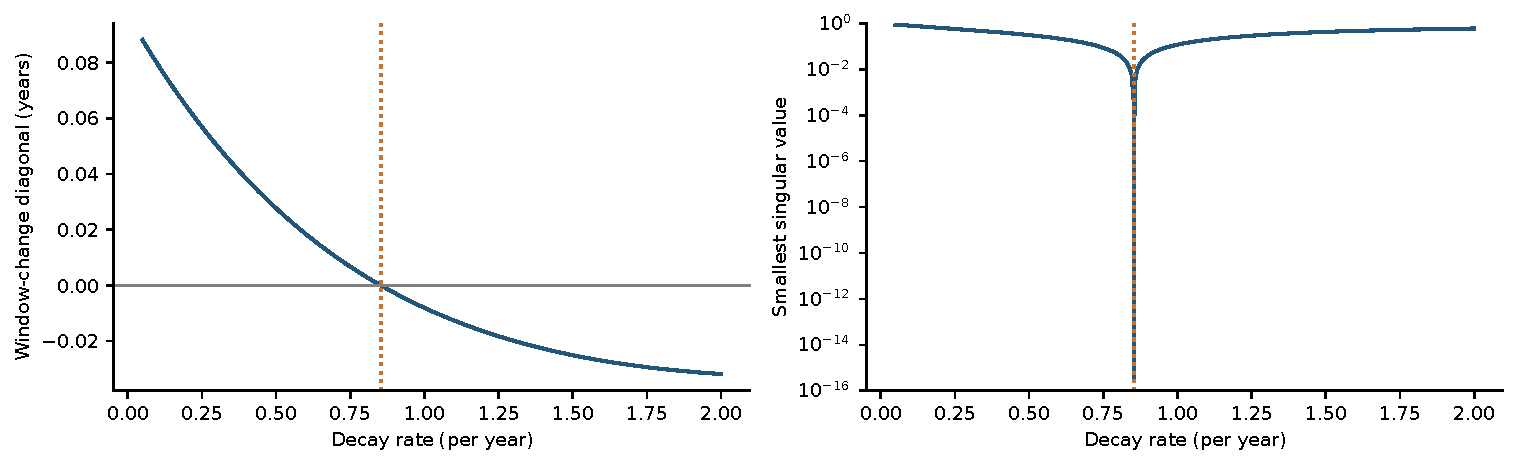
\includegraphics[width=.96\textwidth]{figures/critical_shape.pdf}
\caption{The same calendar can identify at one loading and fail at another. Left: either window-change diagonal in the eight-cell background matrix, in years. Right: smallest singular value of the meeting-free matrix after scaling each background column to unit Euclidean norm. The dotted line marks $\kappa^*$. The normalization removes arbitrary column units, not the loss of information.}\label{fig:criticalshape}
\end{figure}

\subsection{Futures means restore rank, but can add very little precision}
For the same ideal panel and parallel loadings, a calendar-quarter background has rank 23 of 24 columns, and a cell at every meeting has rank 24 of 33. Stacking the additional mean rows \eqref{eq:zrows} gives full column rank in both cases, and with a separate background rate in every expiry gap. These finite-matrix statements are reproduced in the accompanying calendar example.

An explicit confounding direction shows the scale of the extra information. Start with all meeting variances equal to $100$ bp$^2$ and background rates equal to $2500$ bp$^2$/year on the meeting-date partition. Increase the rate on 18 March--29 April 2026 by $360$ bp$^2$/year, and decrease the 18 March and 29 April meeting variances by $23$ and $19$ bp$^2$, respectively. Every option-variance row is unchanged: the affected cell contributes 23 days before the April expiry and 19 days in the next gap. Yet the mean adjustment $z$ changes by at most $1.86\times10^{-9}$ over the panel. For a quarterly future a 0.5 bp rate error changes $\log G_0$ by about $1.3\times10^{-5}$. Thus full rank of the richer observation matrix does not imply useful resolution at that precision. The calculation concerns the additional $z$ rows; known-curve $p$ rows are a further observation set.
